% answers.tex —— 2021 年·全国乙卷·文科 · 参考答案与详细解析片段
% 由 tools/generate_projects.py 依来源总账自 2021/2021_数学真题_全国乙文_试题.md + 2021/2021_数学真题_全国乙文_解析正文.md + 2021/2021_数学真题_全国乙文_答案要点.md 生成，勿手改（改源 MD 后重跑）


\begin{gknotice}
\textbf{解析归属}：下列答案与解析由本库依据试题独立推导，非官方答案；题面核对以指定 PDF 为准。
\end{gknotice}

\gkpart{一、选择题}

\begin{answer}
\gksolhead{1}{}

\textbf{题目}：

已知全集 $U=\{1,2,3,4,5\}$，集合 $M=\{1,2\}$，$N=\{3,4\}$，则 $\complement_U(M\cup N)=$\mbox{（　　）}

\begin{gkopts}(4)
\task A．$\{5\}$
\task B．$\{1,2\}$
\task C．$\{3,4\}$
\task D．$\{1,2,3,4\}$
\end{gkopts}

\Needspace{4\baselineskip}
\textbf{解析}

$M\cup N=\{1,2,3,4\}$，$U$ 中不属于该并集的元素只有 $5$。

\gkanswer{答案：A}

\end{answer}
\begin{answer}
\gksolhead{2}{}

\textbf{题目}：

设 $\mathrm iz=4+3\mathrm i$，则 $z=$\mbox{（　　）}

\begin{gkopts}(4)
\task A．$-3-4\mathrm i$
\task B．$-3+4\mathrm i$
\task C．$3-4\mathrm i$
\task D．$3+4\mathrm i$
\end{gkopts}

\Needspace{4\baselineskip}
\textbf{解析}

\Needspace{5\baselineskip}
由 $\dfrac1{\mathrm i}=-\mathrm i$，
\nopagebreak[4]
\[
z=\frac{4+3\mathrm i}{\mathrm i}=(4+3\mathrm i)(-\mathrm i)=3-4\mathrm i.
\]

\gkanswer{答案：C}

\end{answer}
\begin{answer}
\gksolhead{3}{}

\textbf{题目}：

已知命题 $p:\exists x\in\mathbf R,\ \sin x<1$；命题 $q:\forall x\in\mathbf R,\ \mathrm e^{|x|}\geqslant1$，则下列命题中为真命题的是\mbox{（　　）}

\begin{gkopts}(4)
\task A．$p\land q$
\task B．$\neg p\land q$
\task C．$p\land\neg q$
\task D．$\neg(p\lor q)$
\end{gkopts}

\Needspace{4\baselineskip}
\textbf{解析}

取 $x=0$ 得 $\sin x=0<1$，所以 $p$ 为真命题。又 $|x|\geqslant0$，故 $\mathrm e^{|x|}\geqslant1$ 对任意实数 $x$ 成立，$q$ 也为真命题。

\gkanswer{答案：A}

\end{answer}
\begin{answer}
\gksolhead{4}{}

\textbf{题目}：

函数 $f(x)=\sin\dfrac{x}{3}+\cos\dfrac{x}{3}$ 的最小正周期和最大值分别是\mbox{（　　）}

\begin{gkopts}(2)
\task A．$3\pi$ 和 $\sqrt2$
\task B．$3\pi$ 和 $2$
\task C．$6\pi$ 和 $\sqrt2$
\task D．$6\pi$ 和 $2$
\end{gkopts}

\Needspace{4\baselineskip}
\textbf{解析}

\Needspace{5\baselineskip}
$\sin\frac x3$ 与 $\cos\frac x3$ 的周期均为 $6\pi$，故和函数的最小正周期为 $6\pi$。利用
\nopagebreak[4]
\[
\sin\frac x3+\cos\frac x3=\sqrt2\sin\left(\frac x3+\frac\pi4\right)
\]
可知最大值为 $\sqrt2$，对应选项 C。

\gkanswer{答案：C}

\end{answer}
\begin{answer}
\gksolhead{5}{}

\textbf{题目}：

\Needspace{5\baselineskip}
若 $x,y$ 满足约束条件
\nopagebreak[4]
\[
\begin{cases}
x+y\geqslant4,\\
x-y\leqslant2,\\
y\leqslant3,
\end{cases}
\]
则 $z=3x+y$ 的最小值为\mbox{（　　）}

\begin{gkopts}(4)
\task A．$18$
\task B．$10$
\task C．$6$
\task D．$4$
\end{gkopts}

\Needspace{4\baselineskip}
\textbf{解析}

约束边界的交点为 $(3,1),(1,3),(5,3)$。目标函数在三点的值依次为 $10,6,18$，因此最小值为 $6$。

\gkanswer{答案：C}

\end{answer}
\begin{answer}
\gksolhead{6}{}

\textbf{题目}：

$\cos^2\dfrac{\pi}{12}-\cos^2\dfrac{5\pi}{12}=$\mbox{（　　）}

\begin{gkopts}(2)
\task A．$\dfrac12$
\task B．$\dfrac{\sqrt3}{3}$
\task C．$\dfrac{\sqrt2}{2}$
\task D．$\dfrac{\sqrt3}{2}$
\end{gkopts}

\Needspace{4\baselineskip}
\textbf{解析}

\Needspace{5\baselineskip}
因为 $\cos\frac{5\pi}{12}=\sin\frac\pi{12}$，原式为
\nopagebreak[4]
\[
\cos^2\frac\pi{12}-\sin^2\frac\pi{12}
=\cos\frac\pi6=\frac{\sqrt3}{2}.
\]

\gkanswer{答案：D}

\end{answer}
\begin{answer}
\gksolhead{7}{}

\textbf{题目}：

在区间 $\left(0,\dfrac12\right)$ 随机取一个数，则取到的数小于 $\dfrac13$ 的概率为\mbox{（　　）}

\begin{gkopts}(4)
\task A．$\dfrac34$
\task B．$\dfrac23$
\task C．$\dfrac13$
\task D．$\dfrac16$
\end{gkopts}

\Needspace{4\baselineskip}
\textbf{解析}

\Needspace{5\baselineskip}
均匀分布区间长度为 $\frac12$，满足条件的子区间长度为 $\frac13$，故概率为
\nopagebreak[4]
\[
\frac{1/3}{1/2}=\frac23.
\]

\gkanswer{答案：B}

\end{answer}
\begin{answer}
\gksolhead{8}{}

\textbf{题目}：

下列函数中最小值为 $4$ 的是\mbox{（　　）}

\begin{gkopts}(2)
\task A．$y=x^2+2x+4$
\task B．$y=|\sin x|+\dfrac4{|\sin x|}$
\task C．$y=2^x+2^{2-x}$
\task D．$y=\ln x+\dfrac4{\ln x}$
\end{gkopts}

\Needspace{4\baselineskip}
\textbf{解析}

\Needspace{5\baselineskip}
A 的最小值为 $3$；B 令 $t=|\sin x|\in(0,1]$，则 $t+\frac4t\geqslant4$，实际最小值为 $5$；D 令 $u=\ln x$，当 $u\to0^-$ 时 $u+\frac4u\to-\infty$，不存在最小值。对 C 用基本不等式：
\nopagebreak[4]
\[
2^x+2^{2-x}\geqslant2\sqrt{2^x2^{2-x}}=4,
\]
且 $x=1$ 时取等号。

\gkanswer{答案：C}

\end{answer}
\begin{answer}
\gksolhead{9}{}

\textbf{题目}：

设函数 $f(x)=\dfrac{1-x}{1+x}$，则下列函数中是奇函数的是\mbox{（　　）}

\begin{gkopts}(4)
\task A．$f(x-1)-1$
\task B．$f(x-1)+1$
\task C．$f(x+1)-1$
\task D．$f(x+1)+1$
\end{gkopts}

\Needspace{4\baselineskip}
\textbf{解析}

\nopagebreak[4]
\[
f(x-1)+1=\frac{1-(x-1)}{1+(x-1)}+1=\frac{2-x}{x}+1=\frac2x.
\]
其定义域关于原点对称，且 $g(-x)=-g(x)$，所以该函数为奇函数。

\gkanswer{答案：B}

\end{answer}
\begin{answer}
\gksolhead{10}{}

\textbf{题目}：

在正方体 $ABCD-A_1B_1C_1D_1$ 中，$P$ 为 $B_1D_1$ 的中点，则直线 $PB$ 与 $AD_1$ 所成的角为\mbox{（　　）}

\begin{gkopts}(4)
\task A．$\dfrac{\pi}{2}$
\task B．$\dfrac{\pi}{3}$
\task C．$\dfrac{\pi}{4}$
\task D．$\dfrac{\pi}{6}$
\end{gkopts}

\Needspace{4\baselineskip}
\textbf{解析}

设棱长为 $1$，取 $A=(0,0,0),B=(1,0,0),D_1=(0,1,1)$，则
\Needspace{5\baselineskip}
$P=(\frac12,\frac12,1)$。可取方向向量
\nopagebreak[4]
\[
\overrightarrow{PB}=\left(\frac12,-\frac12,-1\right),\qquad
\overrightarrow{AD_1}=(0,1,1).
\]
两向量点积为 $-\frac32$，模的乘积为 $\sqrt{\frac32}\sqrt2=\sqrt3$，故两直线夹角 $\theta$ 满足 $\cos\theta=\frac{\sqrt3}{2}$，即 $\theta=\frac\pi6$。

\gkanswer{答案：D}

\end{answer}
\begin{answer}
\gksolhead{11}{}

\textbf{题目}：

设 $B$ 是椭圆 $C:\dfrac{x^2}{5}+y^2=1$ 的上顶点，点 $P$ 在 $C$ 上，则 $|PB|$ 的最大值是\mbox{（　　）}

\begin{gkopts}(4)
\task A．$\dfrac52$
\task B．$\sqrt6$
\task C．$\sqrt5$
\task D．$2$
\end{gkopts}

\Needspace{4\baselineskip}
\textbf{解析}

\Needspace{5\baselineskip}
令 $P=(x,y)$。由椭圆方程，$x^2=5(1-y^2)$，所以
\nopagebreak[4]
\[
|PB|^2=x^2+(y-1)^2=6-4y^2-2y
=\frac{25}{4}-4\left(y+\frac14\right)^2.
\]
当 $y=-\frac14$ 时取最大值 $\frac{25}{4}$，故最大距离为 $\frac52$。

\gkanswer{答案：A}

\end{answer}
\begin{answer}
\gksolhead{12}{}

\textbf{题目}：

设 $a\ne0$，若 $x=a$ 是函数 $f(x)=a(x-a)^2(x-b)$ 的极大值点，则\mbox{（　　）}

\begin{gkopts}(4)
\task A．$a<b$
\task B．$a>b$
\task C．$ab<a^2$
\task D．$ab>a^2$
\end{gkopts}

\enlargethispage{2cm}

\Needspace{4\baselineskip}
\textbf{解析}

\nopagebreak[4]
\[
f'(x)=a(x-a)(3x-a-2b),\qquad f''(a)=2a(a-b).
\]
由于 $a\ne0$，$x=a$ 为极大值点当且仅当 $f''(a)<0$，即 $a(a-b)<0$，等价于 $ab>a^2$。

\gkanswer{答案：D}

\end{answer}
\gkpart{二、填空题}

\begin{answer}
\gksolhead{13}{}

\textbf{题目}：

已知向量 $\boldsymbol a=(2,5)$，$\boldsymbol b=(\lambda,4)$，若 $\boldsymbol a\parallel\boldsymbol b$，则 $\lambda=$ \gkblank{}．

\Needspace{4\baselineskip}
\textbf{解析}

\Needspace{5\baselineskip}
二维向量平行的行列式为 $0$：
\nopagebreak[4]
\[
\begin{vmatrix}2&5\\\lambda&4\end{vmatrix}=8-5\lambda=0,
\]
所以 $\lambda=\frac85$。

\gkanswer{答案：$\dfrac85$}

\end{answer}
\begin{answer}
\gksolhead{14}{}

\textbf{题目}：

双曲线 $\dfrac{x^2}{4}-\dfrac{y^2}{5}=1$ 的右焦点到直线 $x+2y-8=0$ 的距离为 \gkblank{}．

\Needspace{4\baselineskip}
\textbf{解析}

\Needspace{5\baselineskip}
双曲线的焦半径参数满足 $c^2=4+5=9$，右焦点为 $(3,0)$。点到直线的距离为
\nopagebreak[4]
\[
\frac{|3+2\cdot0-8|}{\sqrt{1^2+2^2}}=\sqrt5.
\]

\gkanswer{答案：$\sqrt5$}

\end{answer}
\begin{answer}
\gksolhead{15}{}

\textbf{题目}：

记 $\triangle ABC$ 的内角 $A,B,C$ 的对边分别为 $a,b,c$，面积为 $\sqrt3$，$B=60^\circ$，$a^2+c^2=3ac$，则 $b=$ \gkblank{}．

\Needspace{4\baselineskip}
\textbf{解析}

\Needspace{5\baselineskip}
面积关系给出
\nopagebreak[4]
\[
\frac12ac\sin60^\circ=\sqrt3\quad\Longrightarrow\quad ac=4.
\]
\Needspace{5\baselineskip}
再由余弦定理及 $a^2+c^2=3ac$，
\nopagebreak[4]
\[
b^2=a^2+c^2-2ac\cos60^\circ=3ac-ac=2ac=8,
\]
所以 $b=2\sqrt2$。

\gkanswer{答案：$2\sqrt2$}

\end{answer}
\begin{answer}
\gksolhead{16}{}

\textbf{题目}：

以图①为正视图，在图②③④⑤中选两个分别作为侧视图和俯视图，组成某个三棱锥的三视图，则所选侧视图和俯视图的编号依次为 \gkblank{}．（写出符合要求的一组答案即可）
\nopagebreak[4]
\begin{center}% 2021 全国乙卷文科第 16 题：正视图及侧视图、俯视图候选。
% 按指定 PDF 第 1 页（印刷页 1143）重绘；图①尺寸 2×1，图②—③为 2×1，
% 图④—⑤为 2×2。②的中线为实线、③为虚线；④—⑤的水平中线均为实线。
\begin{tikzpicture}[
  x=0.8cm, y=0.8cm,
  font=\small,
  line width=0.45pt,
  line cap=round,
  line join=round
]
  % 图①：直角三角形正视图，底边 2、高 1。
  \begin{scope}[shift={(0,4.2)}]
    \draw (0,0) -- (2,0) -- (2,1) -- cycle;
    \draw (0,-0.38) -- (2,-0.38)
      node[midway, fill=white, inner sep=1pt] {$2$};
    \draw (0,-0.08) -- (0,-0.48);
    \draw (2,-0.08) -- (2,-0.48);
    \draw (2.34,0) -- (2.34,1)
      node[midway, right=2pt, fill=white, inner sep=1pt] {$1$};
    \draw (2.02,0) -- (2.44,0);
    \draw (2.02,1) -- (2.44,1);
    \node[anchor=north] at (1,-0.66) {图①};
  \end{scope}

  % 图②：侧视图候选，中线为实线。
  \begin{scope}[shift={(3.25,4.2)}]
    \draw (0,0) -- (2,0) -- (1,1) -- cycle;
    \draw (1,1) -- (1,0);
    \draw (0,-0.38) -- (2,-0.38)
      node[midway, fill=white, inner sep=1pt] {$2$};
    \draw (0,-0.08) -- (0,-0.48);
    \draw (2,-0.08) -- (2,-0.48);
    \draw (2.34,0) -- (2.34,1)
      node[midway, right=2pt, fill=white, inner sep=1pt] {$1$};
    \draw (2.02,0) -- (2.44,0);
    \draw (2.02,1) -- (2.44,1);
    \node[anchor=north] at (1,-0.66) {图②};
  \end{scope}

  % 图③：侧视图候选，中线为虚线。
  \begin{scope}[shift={(6.5,4.2)}]
    \draw (0,0) -- (2,0) -- (1,1) -- cycle;
    \draw[dashed] (1,1) -- (1,0);
    \draw (0,-0.38) -- (2,-0.38)
      node[midway, fill=white, inner sep=1pt] {$2$};
    \draw (0,-0.08) -- (0,-0.48);
    \draw (2,-0.08) -- (2,-0.48);
    \draw (2.34,0) -- (2.34,1)
      node[midway, right=2pt, fill=white, inner sep=1pt] {$1$};
    \draw (2.02,0) -- (2.44,0);
    \draw (2.02,1) -- (2.44,1);
    \node[anchor=north] at (1,-0.66) {图③};
  \end{scope}

  % 图④：俯视图候选，竖边在左。
  \begin{scope}[shift={(2.0,0)}]
    \draw (0,0) -- (2,1) -- (0,2) -- cycle;
    \draw (0,1) -- (2,1);
    \draw (0,-0.38) -- (2,-0.38)
      node[midway, fill=white, inner sep=1pt] {$2$};
    \draw (0,-0.08) -- (0,-0.48);
    \draw (2,-0.08) -- (2,-0.48);
    \draw (-0.38,0) -- (-0.38,2)
      node[midway, left=2pt, fill=white, inner sep=1pt] {$2$};
    \draw (-0.48,0) -- (0.08,0);
    \draw (-0.48,2) -- (0.08,2);
    \node[anchor=north] at (1,-0.66) {图④};
  \end{scope}

  % 图⑤：俯视图候选，竖边在右。
  \begin{scope}[shift={(5.25,0)}]
    \draw (2,0) -- (0,1) -- (2,2) -- cycle;
    \draw (0,1) -- (2,1);
    \draw (0,-0.38) -- (2,-0.38)
      node[midway, fill=white, inner sep=1pt] {$2$};
    \draw (0,-0.08) -- (0,-0.48);
    \draw (2,-0.08) -- (2,-0.48);
    \draw (2.38,0) -- (2.38,2)
      node[midway, right=2pt, fill=white, inner sep=1pt] {$2$};
    \draw (1.92,0) -- (2.48,0);
    \draw (1.92,2) -- (2.48,2);
    \node[anchor=north] at (1,-0.66) {图⑤};
  \end{scope}
\end{tikzpicture}
\end{center}
\nopagebreak[4]
\Needspace{4\baselineskip}
\textbf{解析}

\Needspace{5\baselineskip}
给出一个满足三视图的三棱锥构造：
\nopagebreak[4]
\[
A=(0,1,0),\quad B=(2,0,0),\quad C=(2,2,0),\quad P=(2,1,1).
\]
取底面顶点 $A=(0,1,0),B=(2,0,0),C=(2,2,0)$、顶点 $P=(2,1,1)$。正视投影为图①；按通常左视图约定，从左侧投影得到图②，俯视投影得到图⑤，故一组答案为②⑤。若从相反侧观察，棱 $AP$ 被遮挡，侧视图为图③。

\gkanswer{答案：②⑤}

\end{answer}
\gkpart{三、解答题}

\begin{answer}
\gksolhead{17}{}

\textbf{题目}：

某厂研制了一种生产高精产品的设备，为检验新设备生产产品的某项指标有无提高，用一台旧设备和一台新设备各生产了 $10$ 件产品，得到各件产品该项指标数据如下：

\begin{center}
\begin{tabular}{cl}
\toprule
设备 & 指标数据 \\
\midrule
旧设备 & $9.8,\ 10.3,\ 10.0,\ 10.2,\ 9.9,\ 9.8,\ 10.0,\ 10.1,\ 10.2,\ 9.7$ \\
新设备 & $10.1,\ 10.4,\ 10.1,\ 10.0,\ 10.1,\ 10.3,\ 10.6,\ 10.5,\ 10.4,\ 10.5$ \\
\bottomrule
\end{tabular}
\end{center}

旧设备和新设备生产产品的该项指标的样本平均值分别记为 $\bar x$ 和 $\bar y$，样本方差分别记为 $s_1^2$ 和 $s_2^2$。

(1) 求 $\bar x,\bar y,s_1^2,s_2^2$；

(2) 判断新设备生产产品的该项指标的均值较旧设备是否有显著提高（如果 $\bar y-\bar x\geqslant2\sqrt{\dfrac{s_1^2+s_2^2}{10}}$，则认为新设备生产产品的该项指标的均值较旧设备有显著提高，否则不认为有显著提高）。

\Needspace{4\baselineskip}
\textbf{解析}

\textbf{(1)}

\Needspace{5\baselineskip}
旧设备数据之和为 $100$，故 $\bar x=10$。其离均差平方和为 $0.36$，所以
\nopagebreak[4]
\[
s_1^2=\frac{0.36}{10}=0.036.
\]
\Needspace{5\baselineskip}
新设备数据之和为 $103$，故 $\bar y=10.3$。其离均差平方和为 $0.40$，所以
\nopagebreak[4]
\[
s_2^2=\frac{0.40}{10}=0.04.
\]

\Needspace{5\baselineskip}
\textbf{(2)}

\nopagebreak[4]
\[
\bar y-\bar x=0.3,\qquad
2\sqrt{\frac{s_1^2+s_2^2}{10}}
=2\sqrt{\frac{0.036+0.04}{10}}
=\frac{\sqrt{19}}{25}\approx0.1744.
\]
因为 $0.3\geqslant\frac{\sqrt{19}}{25}$，按题设判据，新设备的该项指标均值较旧设备有显著提高。

\gkanswer{答案（1）：$\bar x=10,\ \bar y=10.3,\ s_1^2=0.036,\ s_2^2=0.04$}

\gkanswer{答案（2）：有显著提高。}

\end{answer}
\begin{answer}
\gksolhead{18}{}

\textbf{题目}：

如图，四棱锥 $P-ABCD$ 的底面是矩形，$PD\perp$ 底面 $ABCD$，$M$ 为 $BC$ 的中点，且 $PB\perp AM$。
\nopagebreak[4]
\begin{center}% 2021 全国乙卷文科第 18 题：四棱锥 P-ABCD，底面矩形，M 为 BC 中点。
% 按指定 PDF 第 1 页（印刷页 1143）重绘；隐藏棱 PD、DA、DC 与辅助线 AM 用虚线。
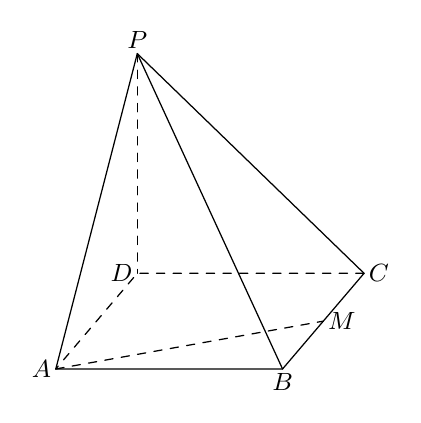
\begin{tikzpicture}[
  x=0.9cm, y=0.9cm,
  font=\small,
  line width=0.45pt,
  line cap=round,
  line join=round,
  every node/.style={inner sep=1.5pt}
]
  \coordinate (A) at (0,0);
  \coordinate (B) at (3.2,0);
  \coordinate (C) at (4.35,1.35);
  \coordinate (D) at (1.15,1.35);
  \coordinate (P) at (1.15,4.45);
  \coordinate (M) at (3.775,0.675);

  % 锥面棱。
  \draw (P) -- (A);
  \draw (P) -- (B);
  \draw (P) -- (C);
  \draw[dashed] (P) -- (D);

  % 矩形底面。
  \draw (A) -- (B) -- (C);
  \draw[dashed] (C) -- (D) -- (A);

  % 题设辅助线 AM。
  \draw[dashed] (A) -- (M);

  \node[anchor=east] at (A) {$A$};
  \node[anchor=north] at (B) {$B$};
  \node[anchor=west] at (C) {$C$};
  \node[anchor=east] at (D) {$D$};
  \node[anchor=south] at (P) {$P$};
  \node[anchor=west] at (M) {$M$};
\end{tikzpicture}
\end{center}
\nopagebreak[4]
(1) 证明：平面 $PAM\perp$ 平面 $PBD$；

(2) 若 $PD=DC=1$，求四棱锥 $P-ABCD$ 的体积。

\Needspace{4\baselineskip}
\textbf{解析}

\gksubpart{(1)}

\Needspace{5\baselineskip}
设 $AB=DC=u>0$，$AD=BC=v>0$，$PD=h>0$。取
\nopagebreak[4]
\[
A=(0,0,0),\ B=(u,0,0),\ C=(u,v,0),\ D=(0,v,0),\
P=(0,v,h),\ M=\left(u,\frac v2,0\right).
\]
\Needspace{5\baselineskip}
由 $\overrightarrow{PB}\perp\overrightarrow{AM}$，
\nopagebreak[4]
\[
\overrightarrow{PB}\cdot\overrightarrow{AM}
=(u,-v,-h)\cdot\left(u,\frac v2,0\right)
=u^2-\frac{v^2}{2}=0.
\]
\Needspace{5\baselineskip}
分别取平面 $PAM$、$PBD$ 的法向量
\nopagebreak[4]
\[
\boldsymbol n_1=\overrightarrow{AP}\times\overrightarrow{AM}
=\left(-\frac{hv}{2},hu,-uv\right),\qquad
\boldsymbol n_2=\overrightarrow{DB}\times\overrightarrow{DP}
=(-hv,-hu,0).
\]
\Needspace{5\baselineskip}
于是
\nopagebreak[4]
\[
\boldsymbol n_1\cdot\boldsymbol n_2
=\frac{h^2v^2}{2}-h^2u^2=0.
\]
两平面的法向量垂直，故平面 $PAM\perp$ 平面 $PBD$。

\gksubpart{(2)}

\Needspace{5\baselineskip}
由 $DC=u=1$ 及 $u^2=\frac{v^2}{2}$ 得 $v=\sqrt2$，矩形底面积为 $uv=\sqrt2$。高 $PD=1$，所以
\nopagebreak[4]
\[
V_{P-ABCD}=\frac13\cdot\sqrt2\cdot1=\frac{\sqrt2}{3}.
\]

\gkanswer{答案（1）：见解析版}

\gkanswer{答案（2）：$\dfrac{\sqrt2}{3}$}

\end{answer}
\begin{answer}
\gksolhead{19}{}

\textbf{题目}：

设 $\{a_n\}$ 是首项为 $1$ 的等比数列，数列 $\{b_n\}$ 满足 $b_n=\dfrac{na_n}{3}$。已知 $a_1,3a_2,9a_3$ 成等差数列。

(1) 求 $\{a_n\}$ 和 $\{b_n\}$ 的通项公式；

(2) 记 $S_n$ 和 $T_n$ 分别为 $\{a_n\}$ 和 $\{b_n\}$ 的前 $n$ 项和，证明 $T_n<\dfrac{S_n}{2}$。

\Needspace{0.4\textheight}

\Needspace{4\baselineskip}
\textbf{解析}

\gksubpart{(1)}

\Needspace{5\baselineskip}
设等比数列公比为 $q$。由 $a_1=1$ 及 $a_1,3a_2,9a_3$ 成等差数列，
\nopagebreak[4]
\[
2(3q)=1+9q^2\quad\Longrightarrow\quad(3q-1)^2=0,
\]
\Needspace{5\baselineskip}
故 $q=\frac13$，从而
\nopagebreak[4]
\[
a_n=3^{1-n},\qquad b_n=\frac{na_n}{3}=\frac{n}{3^n}.
\]

\gksubpart{(2)}

\nopagebreak[4]
\[
S_n=\frac32(1-3^{-n}),\qquad
T_n=\sum_{k=1}^n\frac{k}{3^k}
=\frac34\left(1-\frac{n+1}{3^n}+\frac{n}{3^{n+1}}\right).
\]
\Needspace{5\baselineskip}
因此
\nopagebreak[4]
\[
\frac{S_n}{2}-T_n
=\frac{n}{2\cdot3^n}>0\quad(n\geqslant1),
\]
即 $T_n<\frac{S_n}{2}$。

\gkanswer{答案（1）：$a_n=3^{1-n},\quad b_n=\dfrac{n}{3^n}$}

\gkanswer{答案（2）：见解析版}

\end{answer}
\begin{answer}
\gksolhead{20}{}

\textbf{题目}：

已知抛物线 $C:y^2=2px\ (p>0)$ 的焦点 $F$ 到准线的距离为 $2$。

(1) 求 $C$ 的方程；

(2) 已知 $O$ 为坐标原点，点 $P$ 在 $C$ 上，点 $Q$ 满足 $\overrightarrow{PQ}=9\overrightarrow{QF}$，求直线 $OQ$ 斜率的最大值。

\Needspace{4\baselineskip}
\textbf{解析}

\gksubpart{(1)}

\Needspace{5\baselineskip}
抛物线 $y^2=2px$ 的焦点为 $(\frac p2,0)$，准线为 $x=-\frac p2$，焦点到准线的距离为 $p$。由 $p=2$ 得
\nopagebreak[4]
\[
C:y^2=4x.
\]

\gksubpart{(2)}

\Needspace{5\baselineskip}
令 $P=(t^2,2t)$，焦点 $F=(1,0)$。由向量等式
\nopagebreak[4]
\[
\overrightarrow{PQ}=9\overrightarrow{QF}
\]
\Needspace{5\baselineskip}
得 $Q-P=9(F-Q)$，即 $Q=\frac{P+9F}{10}$。于是
\nopagebreak[4]
\[
Q=\left(\frac{t^2+9}{10},\frac t5\right),\qquad
k_{OQ}=\frac{2t}{t^2+9}.
\]
由 $(t-3)^2\geqslant0$ 可得 $\frac{2t}{t^2+9}\leqslant\frac13$，等号在 $t=3$ 时成立，故最大斜率为 $\frac13$。

\gkanswer{答案（1）：$y^2=4x$}

\gkanswer{答案（2）：$\dfrac13$}

\end{answer}
\begin{answer}
\gksolhead{21}{}

\textbf{题目}：

设函数 $f(x)=x^3-x^2+ax+1$。

(1) 讨论 $f(x)$ 的单调性；

(2) 求曲线 $y=f(x)$ 过坐标原点的切线与曲线 $y=f(x)$ 的公共点的坐标。

\Needspace{4\baselineskip}
\textbf{解析}

\gksubpart{(1)}

\nopagebreak[4]
\[
f'(x)=3x^2-2x+a.
\]
当 $a\geqslant\frac13$ 时，$f'(x)\geqslant0$ 对所有 $x$ 成立，且仅可能在单点取零，故 $f$ 在 $\mathbf R$ 上递增。

\Needspace{5\baselineskip}
当 $a<\frac13$ 时，$f'(x)=0$ 的两根为
\nopagebreak[4]
\[
x_1=\frac{1-\sqrt{1-3a}}3,\qquad x_2=\frac{1+\sqrt{1-3a}}3.
\]
导数在两根外为正、两根之间为负，故 $f$ 在 $(-\infty,x_1)$、$(x_2,+\infty)$ 上递增，在 $(x_1,x_2)$ 上递减。

\gksubpart{(2)}

\Needspace{5\baselineskip}
设过原点的切点横坐标为 $t$。切线方程为 $y=f'(t)(x-t)+f(t)$，过原点要求
\nopagebreak[4]
\[
f(t)-tf'(t)=-2t^3+t^2+1=0
=-(t-1)(2t^2+t+1)=0.
\]
\Needspace{5\baselineskip}
二次因式无实根，故 $t=1$。切线斜率为 $f'(1)=a+1$，切线方程为 $y=(a+1)x$。与曲线联立：
\nopagebreak[4]
\[
x^3-x^2-x+1=(x-1)^2(x+1)=0.
\]
公共点横坐标为 $1,-1$，相应坐标为 $(1,a+1)$、$(-1,-a-1)$。

\Needspace{8\baselineskip}

\gkanswer{答案（1）：$a\geqslant\dfrac13$ 时在 $\mathbf R$ 上递增；若 $a<\dfrac13$，令 $x_1=\dfrac{1-\sqrt{1-3a}}3$、$x_2=\dfrac{1+\sqrt{1-3a}}3$，则在 $(-\infty,x_1)$、$(x_2,+\infty)$ 上递增，在 $(x_1,x_2)$ 上递减。}

\gkanswer{答案（2）：$(1,a+1)$、$(-1,-a-1)$}

\end{answer}
\begin{answer}
\gksolhead{22}{}

\textbf{题目}：

在直角坐标系 $xOy$ 中，$\odot C$ 的圆心为 $C(2,1)$，半径为 $1$。

(1) 写出 $\odot C$ 的一个参数方程；

(2) 过点 $F(4,1)$ 作 $\odot C$ 的两条切线，以坐标原点为极点，$x$ 轴正半轴为极轴建立极坐标系，求这两条切线的极坐标方程。

\Needspace{4\baselineskip}
\textbf{解析}

\gksubpart{(1)}

\Needspace{5\baselineskip}
圆心为 $(2,1)$、半径为 $1$，故一个参数方程为
\nopagebreak[4]
\[
\begin{cases}
x=2+\cos t,\\
y=1+\sin t,
\end{cases}\qquad 0\leqslant t<2\pi.
\]

\gksubpart{(2)}

\Needspace{5\baselineskip}
设过 $F(4,1)$ 的切线斜率为 $m$，方程为 $y-1=m(x-4)$。圆心到直线的距离等于半径：
\nopagebreak[4]
\[
\frac{2|m|}{\sqrt{m^2+1}}=1
\quad\Longrightarrow\quad m=\pm\frac1{\sqrt3}.
\]
\Needspace{5\baselineskip}
两条直线分别化为
\nopagebreak[4]
\[
x-\sqrt3y=4-\sqrt3,\qquad x+\sqrt3y=4+\sqrt3.
\]
\Needspace{5\baselineskip}
代入 $x=r\cos\theta,\ y=r\sin\theta$，得到
\nopagebreak[4]
\[
r(\cos\theta-\sqrt3\sin\theta)=4-\sqrt3,\qquad
r(\cos\theta+\sqrt3\sin\theta)=4+\sqrt3.
\]

\gkanswer{答案（1）：$\begin{cases}x=2+\cos t,\\y=1+\sin t.\end{cases}$}

\gkanswer{答案（2）：$r(\cos\theta-\sqrt3\sin\theta)=4-\sqrt3$，$r(\cos\theta+\sqrt3\sin\theta)=4+\sqrt3$}

\end{answer}
\begin{answer}
\gksolhead{23}{}

\textbf{题目}：

已知函数 $f(x)=|x-a|+|x+3|$。

(1) 当 $a=1$ 时，求不等式 $f(x)\geqslant6$ 的解集；

(2) 若 $f(x)>-a$，求 $a$ 的取值范围。

\makeatletter\def\gkanswerblock{answer}\ifx\@currenvir\gkanswerblock\else\clearpage\fi\makeatother

\Needspace{4\baselineskip}
\textbf{解析}

\gksubpart{(1)}

\Needspace{5\baselineskip}
当 $a=1$ 时，分段得
\nopagebreak[4]
\[
f(x)=
\begin{cases}
-2x-2,&x\leqslant-3,\\
4,&-3\leqslant x\leqslant1,\\
2x+2,&x\geqslant1.
\end{cases}
\]
故 $f(x)\geqslant6$ 等价于 $x\leqslant-4$ 或 $x\geqslant2$，解集为 $(-\infty,-4]\cup[2,+\infty)$。

\gksubpart{(2)}

说明：原题只写“若 $f(x)>-a$”，未明确量词，以下分别讨论全称与存在两种解释。

\Needspace{5\baselineskip}
$f(x)=|x-a|+|x+3|$ 的最小值为两定点 $a,-3$ 的距离 $|a+3|$，且在两点之间可取到。因此恒有 $f(x)>-a$ 等价于
\nopagebreak[4]
\[
|a+3|>-a.
\]
若 $a<-3$，不等式不成立；若 $a\geqslant-3$，则需 $a+3>-a$，故全称解释的范围为 $a>-\frac32$。若只要求存在实数 $x$ 使不等式成立，由 $f(x)\to+\infty$（$|x|\to+\infty$），任意实数 $a$ 都可满足，范围为 $\mathbf R$。

\gkanswer{答案（1）：$(-\infty,-4]\cup[2,+\infty)$}

\gkanswer{答案（2）：全称解释为 $a>-\dfrac32$；存在解释为 $a\in\mathbf R$。}

\end{answer}